\chapter{Introduction}
\begin{quote}
Because it's there.
\end{quote}
\hfill --- George Mallory, when asked why he wanted to climb Mount Everest.\\
\vspace{0.5in}

The idea of an intelligent robot performing a variety of tasks, extraordinary 
and mundane, up to and exceeding human performance, has captured the hearts and 
minds of people since at least the European Renaissance.  A key feature of much 
of this romantic vision is that robots can interact with {\em us}---working 
with, around and for humans.  An understanding of human pose is a crucial 
component to making this compelling dream become a reality.  

In the more practical and not-too-distant future, understanding human pose from 
images has enormous potential to help in many computer vision tasks: semantic 
indexing of images and video~\citep{posesearch}, action 
recognition~\citep{pose-action11}, human-object interaction~\citep{bangpeng12}, 
and scene understanding~\citep{gupta11}, to name a few.   

The problem of human pose understanding is also interesting in its own right.  
It pushes the boundaries of what can and cannot be accomplished by artificially 
intelligent systems.  Infants and even other species can understand human 
pose---why can't a computer?  

Pose estimation subsumes one of the holy grails of computer vision: general 
object recognition.  It serves as useful vehicle to demonstrate computer vision 
techniques that can be used in other subfields.  Humans can be considered a 
collection of related objects (body parts), or a single, highly deformable 
object.  The parts themselves are some of the most difficult to detect in the 
literature.  Typical objects that researchers work on recognizing---faces, 
bicycles or even potted plants \citep{voc09}---have distinguishing features, 
reliable patterns and limited intra-class variability.  A body part such as a 
lower arm, on the other hand, is far more generic.  It has a generic shape---
at best it can be described as a projection of a cylinder or frustum---and is 
subject to much higher intra-class variability due to clothing, articulated 
pose, body type, and severe foreshortening.  Features developed must be 
invariant to pose, lighting, texture and color and still discriminate parts 
from clutter, or efficient search procedures over these variations need to be 
developed. These types of techniques are valuable for computer vision in 
general.

Human pose estimation is also one of the most computationally demanding 
problems in computer vision, as the set of possible outputs is combinatorial in 
the number of parts.  It can be posed as a graph assignment or graphical model 
inference problem with an enormous set of possible labels (for each part, 
determine which pixel it is associated with).  This makes it an interesting 
testbed for advancements in graphical model and matching algorithms for and 
beyond computer vision.

Finally, the problem of pose estimation is timely.  In the computer vision 
community, statistical machine learning tools and supervised datasets give us 
principled protocols to learn effective recognition models which didn't exist a 
decade ago.  Robots, cameras, and automated systems are more and more pervasive 
in everyday life.  The demand for reliable pose estimation is already felt in 
the entertainment and defense industries. 

For all these reasons---practical applications, the dream of artificial 
intelligence, the general applicability to vision and machine learning, the 
convergence of technology to make it all possible---human pose estimation is an 
excellent problem upon which to focus.


\section{Problem Statement}

Here we formalize our problem definition input, output and computational 
requirements as follows:  

\begin{problem}[2D human upper-body pose estimation]
\label{prob:pose}
\hspace*{\fill}
\begin{itemize}
 \item[Input:] A single RGB image or RGB video sequence containing the rough 
location and scale of a person in every frame, with no additional information.
\item[Output:] Line segments describing the major anatomical parts \{left and 
right upper arms, left and right lower arms, torso, head\} in pixel 
coordinates.
\item[Requirements:] Computation time and space polynomial in the number of 
input pixels and number of output parts.
\end{itemize}
\end{problem}

\begin{figure}[tb]
\begin{center}
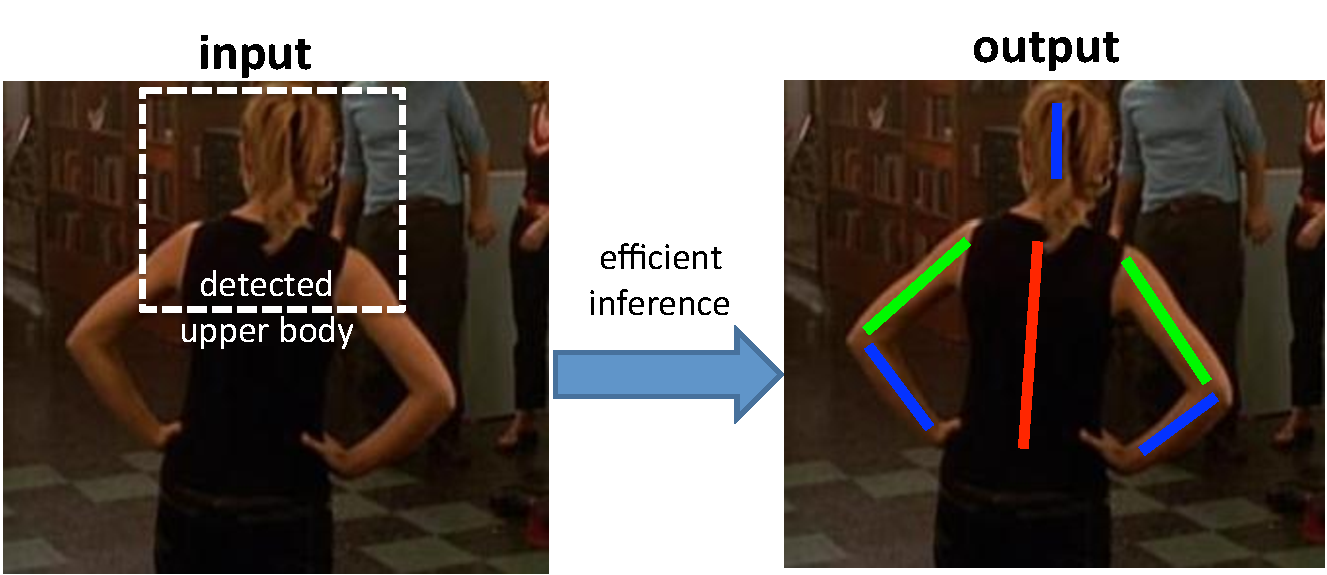
\includegraphics[width=0.95\textwidth]{figs/problem-statement.pdf}
\caption[Statement of problem.]{An example illustrating the pose estimation 
problem, formalized in~\probref{pose}.}
\label{fig:pose-problem}
\end{center}
\end{figure}

Importantly, we concern ourselves only with 2D (two dimensional) input.  This 
makes the task much more challenging than when using additional sensors, such 
as in Microsoft's Kinect capture system~\citep{kinect} where depth information 
and hence reliable knowledge of the background can be used.  However, our 
limited-sensor problem also means it can be applied in more general settings: 
we can apply such pose estimation methods outdoors and on the wealth of 
archival images and footages already stored on personal computers, libraries, 
and photo and video sharing web sites.  

Furthermore, we do not assume any additional information, such as knowledge of 
the foreground, background, clothing, lighting, indoor versus outdoor, 
etcetera.  All these factors work to confound estimation by introducing 
appearance artifacts.  We refer to our general setting as pose estimation {\em 
in the wild}, to stress the fact that the datasets we consider are from 
unconstrained foreground and backgrounds settings (or nearly unconstrained, 
when dealing with TV shows).

Also of note, we only consider the upper body, although all methods and models 
discussed in this work can be extended to full body processing (\ie including 
hips and upper and lower legs).  In fact, most of the models and tools 
developed in this work can be applied to other articulated objects, and in 
general, other domains in which estimating the instantiation of interacting 
parts (\eg, handwriting recognition, or gene sequencing). We focus on upper 
body human pose in this work because (1) most interesting pose variation occurs 
in the upper body, (2) there is a vast amount of data of people's upper bodies 
from TV shows, movies and images where lower halves are not visible, and (3) 
there is little extra knowledge to be learned about pose estimation by 
including the lower body parts, while increasing the computation time of all 
models at least linearly.  

Finally, we restrict ourselves to polynomial running time.  The space of all 
possible poses is exponential in the number of parts. The ideal approach, if 
computation were not an issue, would be to enumerate all possible poses and 
score them all using any scoring function of arbitrary complexity. However, 
this is simply not feasible, and we are forced to make conditional independence 
assumptions between certain parts to achieve tractability.  In practice, we 
wish to estimate pose on the order of a few minutes or seconds per frame.

\section{Intrinsic difficulties}
Human pose estimation in the wild is an extremely challenging problem.  It 
shares all of the difficulties of object detection, such as confounding 
background clutter, lighting, viewpoint, and scale. In addition, there are 
significant difficulties unique to human poses.  We are forced to reason over 
an enormous number of plausible poses for each image, making this a very 
computationally demanding problem.  In this section we go over the intrinsic 
difficulties of this problem, both from perceptual and computational 
standpoints.

\subsection{Perceptual issues}\label{sec:perceptual}
\begin{figure}[tb]
\begin{center}
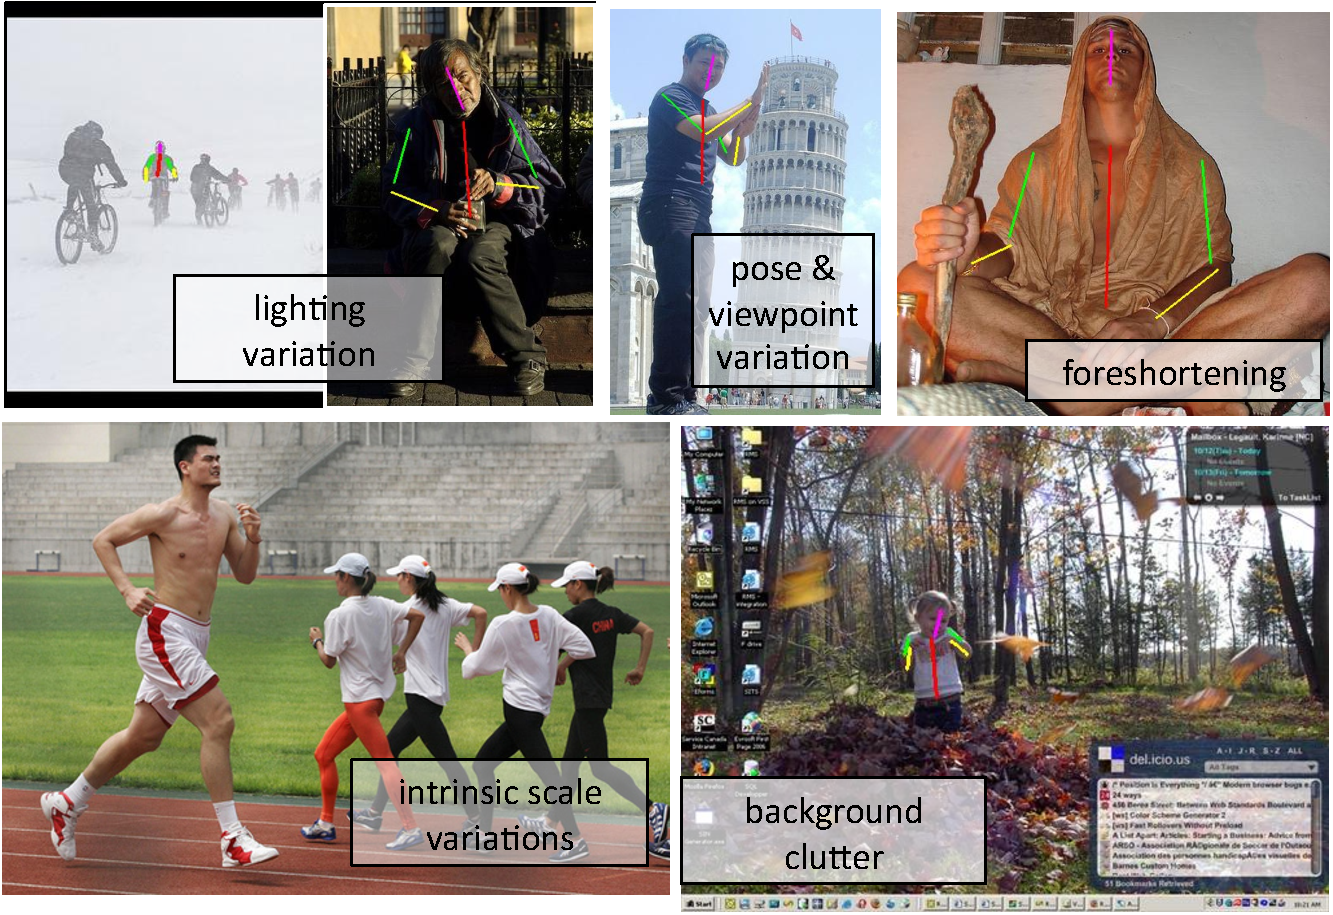
\includegraphics[width=1.05\textwidth]{figs/perceptual-issues.pdf}
\caption[Perceptual difficulties in pose estimation]{Some of the perceptual 
challenges in human pose estimation.  Large variations in lighting, pose, 
viewpoint, foreshortening, relative scale and clutter all work to confound pose 
estimation.  See~\secref{perceptual}}
\label{fig:perceptual-issues}
\end{center}
\end{figure}

One of the primary difficulties in human pose estimation is that appearance of 
pose is largely unconstrained, making it highly variable with multiple 
appearance modes.  The following issues are illustrated 
in~\figref{perceptual-issues}.

\mypar{Lighting:} Images of pose can be taken indoor or outdoor, making not 
only the mean intensity of the image variable (signal bias), but also contrast 
(signal gain). This issue is well studied in computer vision, and to an extent, 
features have been developed to be invariant to lighting, \eg, HoG~\citep{hog}, 
but require harsh quantization and local normalization of edge energy 
information. 

\mypar{Viewpoint and pose: } Humans can look very different depending on where 
they are with respect to the imaging plane.  The global ``twist'' (rotation 
about the length-of-body axis) which determines the degree of frontal versus 
profile stance of the person can be somewhat mitigated by coarse person 
detectors~\citep{andriluka2010}.  However, the body can also go through radical 
appearance changes due to the articulation of the limbs, forcing practical 
systems to decompose the modeling into the most basic, articulation-invariant 
components as atomic units: limbs and joints.

\mypar{Relative scale:} We assume our input is a detected person at a rough 
global scale.  However, we still have a large variation in the scale of parts 
in two different ways: In any particular person, the ratio of limb lengths may 
not be consistent; \eg a baby's proportions are very different than an adult's.  
Across people, there are also a large differences in the geometries of parts, 
based on gender, body type (fat, skinny, muscular), and age.  These further 
contribute to the variability in appearance.

\mypar{2D projection:} The fact that we are working with images that are 
projections of the real world lead to further difficulties.  Foreshortening 
makes estimating the length of the limb in 2D coordinates even more difficult, 
and changes the appearance.  Self-occlusions and foreground occlusions make a 
part invisible and are very hard to determine without further scene or depth 
knowledge.  Finally, it is inherently ambiguous to map from 2D pose to 3D real 
world coordinates (even up to an unknown global scale factor), discussed 
further in~\secref{limitations}.  This makes it difficult to model priors on 
arm length, as we are forced to measure and reason about lengths on the 2D 
pixel grid.

\mypar{Clothing:} Clothing contributes a near-infinite space of foreground 
variation.  Not only is clothing responsible for foreground clutter, it also 
can be considered an occluder which hides parts (\eg baggy clothing, skirts, 
ponchos) and can break assumptions about left-right appearance symmetry (\eg an 
asymmetric shirt).

\mypar{Background clutter:} Background clutter accounts for roughly half the 
errors in pose estimation performance. Often it is extremely difficult to 
separate edges in the background from lower arms.  Lower arms appear as little 
more than a pair of roughly parallel lines in an image, as do many man-made 
structures and natural objects in backgrounds: walls, tables, chairs, posts, 
trees, etcetera.

\begin{figure}[tb]
\begin{center}
\includegraphics[width=1.05\textwidth]{figs/dataset-multimodal.pdf}
\caption[Variations in appearance]{Some illustrations of variation in 
appearance in the PASCAL Stickmen dataset.  (a) An average of the dataset in 
grayscale.  (b) Average of Sobel edges over dataset.  (c) Polar histogram of 
the inner angle made between upper and lower arm, with examples for 
$0^\circ,45^\circ,90^\circ,135^\circ,180^\circ,225^\circ,270^\circ$ and 
$315^\circ$. (d) A random sampling of 100 left elbows from the Buffy Stickmen 
pose dataset,	removing color and intensity bias, to illustrate the huge variety 
of appearance due to	clutter, motion blur, clothing, body type, and pose.  
\label{fig:dataset-multimodal}}
\end{center}
\end{figure}



\subsection{Computational issues}

To operationalize \probref{pose}, let $x$ be the input image pixels, and $y$ be 
a representation of the output predicted pose.  Then a general solution 
to~\probref{pose} would take the form of a {\em scoring function} $s(x,y)$ 
which evaluates the quality of any estimated pose $y$ in the image $x$.  We can 
define the ``best'' pose as the highest scoring: $y^\star = \argmax_y s(x,y)$ 
(or $y^\star = \arg\sup_y s(x,y)$ if $y$ is infinite dimensional, \ie 
continuous).  Then~\probref{pose} is satisfied if this determination of the 
maximizer can be done in polynomial time. There are two sources of intrinsic 
computational complexity within this framework. 

\mypar{Complexity of the input:} For the reasons outlined 
in~\secref{perceptual}, there are an astronomical number of different inputs 
$x$ that can map to the same true pose $y$---the same layout of body parts can 
look very different from image to image.  The problem is inherently multimodal, 
in the sense that radically different appearances are equally valid input 
representations of any particular pose.  For a few different illustrations of 
the variability of a dataset, see~\figref{dataset-multimodal}. 

To deal with this complex problem, we are forced to either design features that 
are invariant to the multimodality (\eg, a generic patch-based arm detector 
based on coarse edges, or geometric features based on relative part coordinate 
systems), or to partition the space and model multiple modes separately.  In 
the case of the latter approach, we are faced with other difficult decisions 
regarding model complexity: how to define modes and a notion of locality, and 
what the right trade-off is between the richness of the model and the error in 
fitting the model at different modes with a finite amount of training data.

\mypar{Complexity of the output:}
The enormous combinatorial space of possible output poses is a second source of 
computational complexity.  A typical discretization of the state space of human 
poses is an $80 \times 80$ spatial grid of part locations at $24$ possible 
angles~\citep{felz05}, resulting in an output space that is roughly $150000$ 
possibilities for each part, and thus $150000^6 \approx 10^{30}$ for the joint 
output space of all $6$ upper body parts~\footnote{In the case of continuous 
spaces, the output space is infinite (infinitely precise), and to maintain 
tractability the form of $s(x,y)$ is typically analytical with a closed-form 
maximum, mean and/or mode, or approximate sampling techniques are used for 
inference. See \secref{rel}.}.

Enumerating all possibilities for a joint configuration of all parts is clearly 
not feasible.  At the other extreme, we could ignore part interactions, and 
estimate the pose of each part separately---a task which instead has $6 \times 
150000$ possibilities, which is computationally very cheap with modern 
computers.  However, individual part detection is extremely difficult for body 
parts~\citep{andriluka09} due to the wide range of appearances and lack of 
discriminating features.

Between the two extremes of (1) estimating parts in isolation and (2) 
enumerating all possible joint pose configurations, there lies a family of 
models $s(x,y)$ that consider {\em some} part interactions, but not all.  The 
simplest of these is a {\em first-order}, or {\em pairwise model}, which looks 
at pairs of part interactions at a time, and the graph of part interactions 
forms a tree structure.  This compromise between a full model of every part and 
a decoupled model of independent parts will be the basic model building block 
throughout this work.

In such a pairwise model, the basic bottleneck operation is to evaluate the 
quality of a pair of parts at a time. The model combines all such pairwise 
scores together to determine the optimal global pose.  This scoring requires 
$150000^2 \approx 1$ billion possibilities to consider for a pair of parts in 
our example $80 \times 80 \times 24$ state space, which is large but just small 
enough for modern machines to handle with some additional model restrictions, 
detailed in~\secref{ps}.


\section{Contributions of this thesis}
\begin{figure}[t!]
\begin{center}
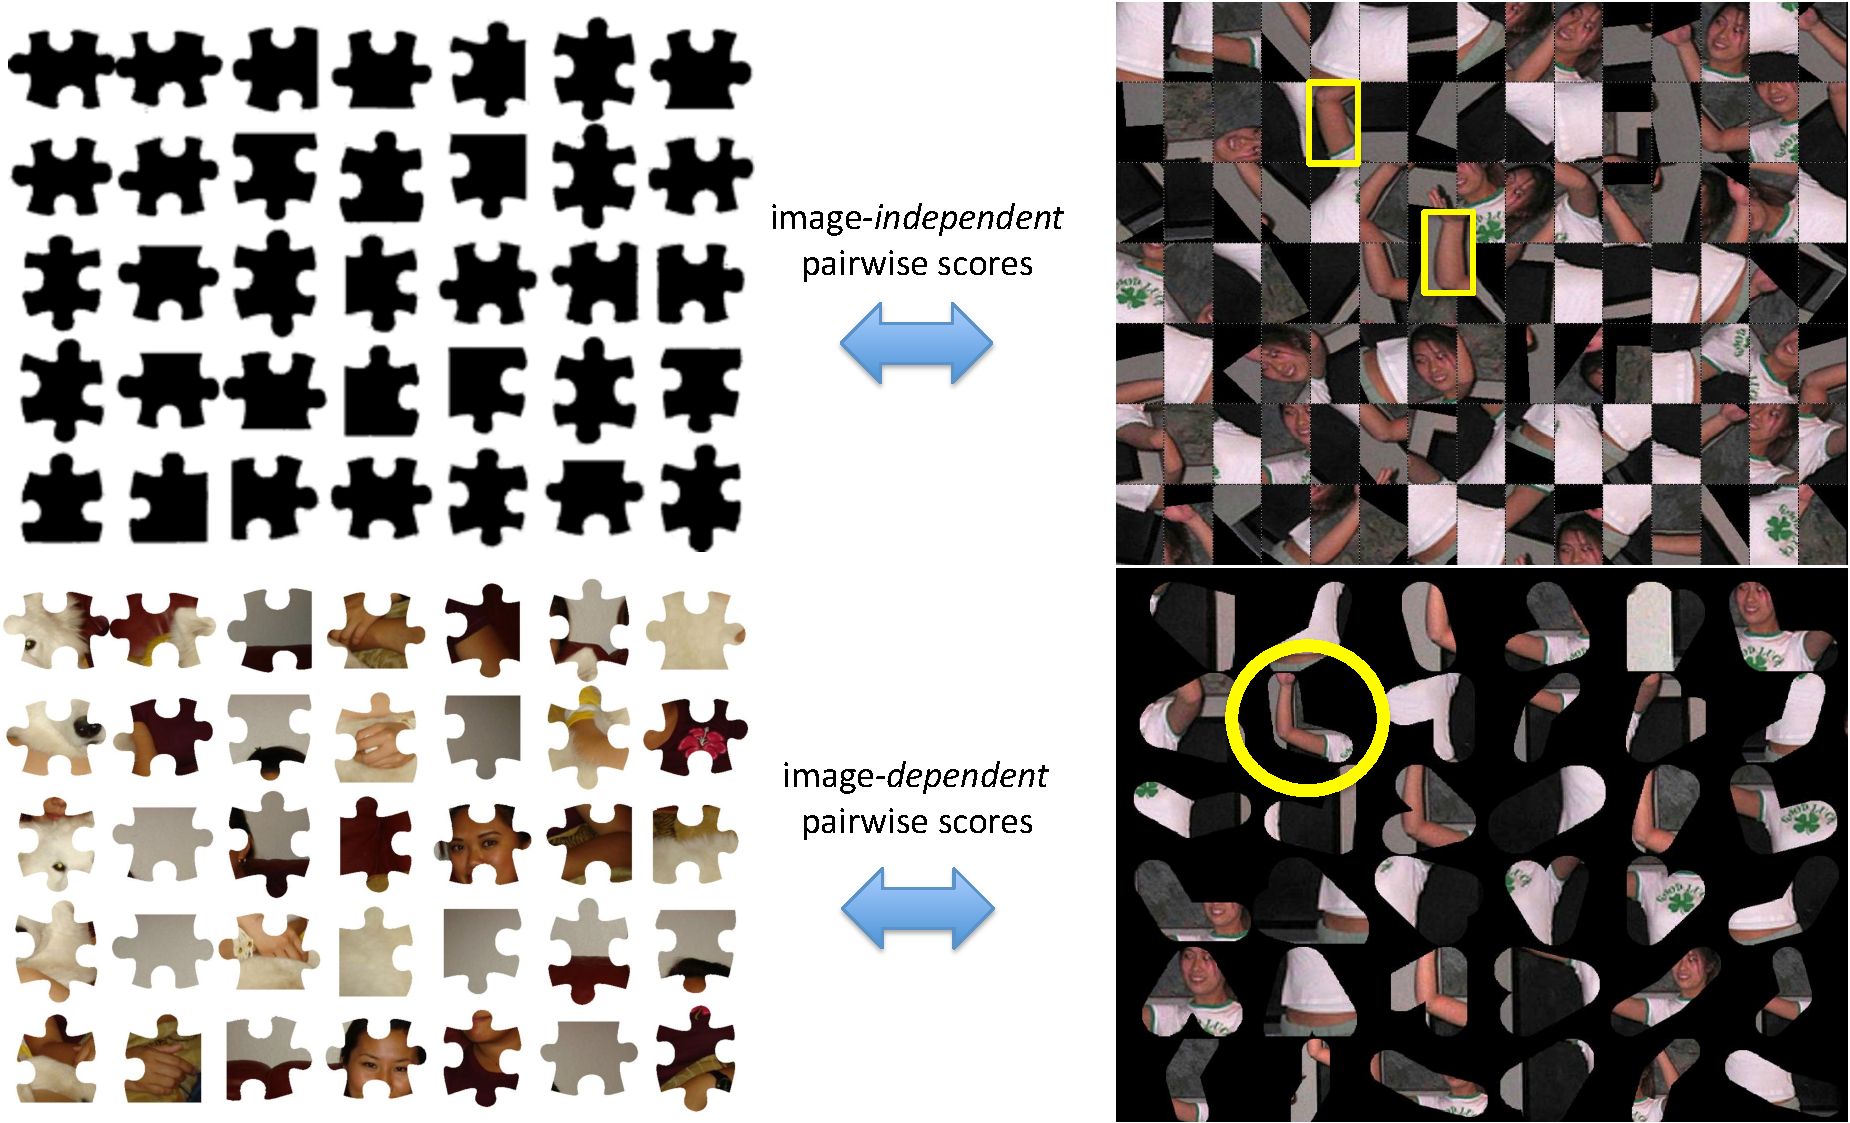
\includegraphics[width=0.99\textwidth]{figs/puzzle.pdf}
\caption[Puzzle analogy of pose estimation.]{Puzzle analogy of pose estimation.  
Classical approaches only use individual part detectors and geometric 
plausibility to determine the pose of a person.  This is analogous to 
attempting to put together a puzzle without looking at appearance of the pieces 
---only the plausibility of them fitting together. On the other hand, models 
with data-dependent interactions are analogous to using the appearance of the 
puzzle piece faces as well as their fit when constructing the puzzle.  Even for 
humans, it is easier to spot the correct pair of upper/lower arms when they are 
examined jointly.}
\label{fig:puzzle}
\end{center}
\end{figure}

Due to the computational issues discussed above, previous work in pose 
estimation has resorted to a model of pose that considers, at most, pairwise 
interactions between parts, in a specially restricted form: the network of 
part-pair interactions is described by a tree structured graph, and the 
interactions are described by simple kinematic consistency.  This is known as 
the basic {\em pictorial structure} (PS) model, also referred to as a {\em 
spring model}---see \secref{ps}, and \figref{spring-model-intro}.  

In PS models, each part has an individual score for placement at any location 
in the image, which must be balanced with part-pair penalties for deforming 
from the default model positions (``pose prior'').  For example, the 
deformation penalty between an upper arm and lower arm expresses the fact that 
they should roughly agree on where the elbow is.  The deformation penalties can 
be thought of as springs at rest at default positions and stretched by moving 
the parts to new positions.  The parts themselves are attracted individually to 
likely spots in the image.  Thus a balance is sought between individual part 
beliefs and respecting the prior notion of what a pose should look like.

\begin{figure}[tb]
\begin{center}
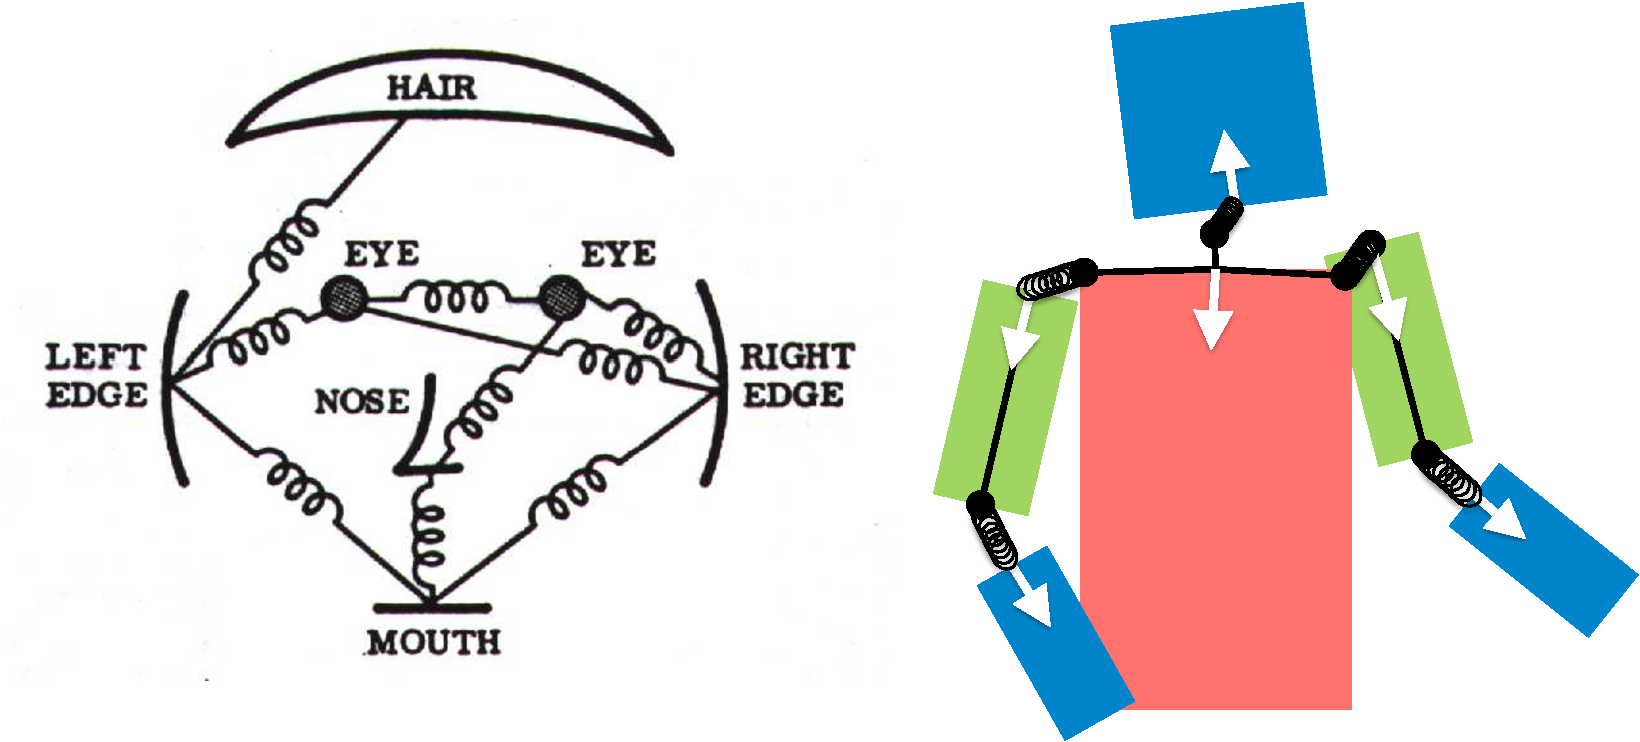
\includegraphics[width=0.99\textwidth]{figs/spring-model.pdf}
\caption[Spring model of pose.]{Spring model of pose.  At left, the original 
spring pictorial structure model that appeared in \citet{fischler1973ps}. At 
right, the standard PS model for 2D human pose.  The states are shown as unit 
vectors indicating the position of joints and their direction.  The mean 
displacement between joints are shown as solid black circles, connected by 
solid black lines to show the kinematic tree structure.  The displacement from 
mean positions are shown as springs stretching.  This figure is repeated again 
for convenience in \secref{ps}.}
\label{fig:spring-model-intro}
\end{center}
\end{figure}


An important property of PS models is that the pairwise, spring stretch, 
termsare {\em blind to the image content}.  The problem with this is that 
individual part detector scores are extremely weak (\secref{perceptual}): they 
must work in isolation and generalize to limbs in all settings of backgrounds, 
foregrounds, articulation, and environment.

As a result, the above model is effectively trying to piece together parts of a 
person, when the parts themselves are extremely ambiguous. As an extreme 
analogy of this, it is similar to attempting to put together a jigsaw puzzle in 
which the pieces themselves are very generic.  One has many plausible 
candidates for where each puzzle piece should go individually (like individual 
part scores), but to determine whether two pieces are adjacent, one can only 
see how well they fit together, and {\em not } the  image content on their 
faces; see \figreff{puzzle}{top row}.


\subsection{Image-dependent interactions in a tree structured 
model,~\secref{CPS}}
\label{sec:contrib1}
As an improvement over the basic PS model, we wish to actually {\em exploit } 
image content when modeling pairwise interactions.  In the puzzle analogy, this 
would allow us to fit pieces together based on their color similarity and 
continuous contours across the connection boundary; see \figreff{puzzle}{bottom 
row}.  We exploit these same cues for determining whether limbs go together in 
an image, as well as additional cues such as region support and multimodal 
descriptions of geometry.

Unfortunately, this turns out to be computationally infeasible using standard 
tools and techniques.  In light of this, we propose a {\em cascade} of models 
to focus computation on pose possibilities that are more promising.  There are 
many pose possibilities that are easy to reject as incorrect with a simple 
model (like a basic PS model, or even simpler), and we are then able to freely 
apply a richer model on the possibilities that remain.  This is illustrated 
in~\figref{cps-overview}.

To employ a cascade approach, we develop and analyze {\em structured prediction 
cascades}, and apply them to the problem of 2D pose estimation. Importantly, we 
provide a novel training objective for the cascade so that parameters of the 
models are learned to specifically to filter out a significant proportion of 
possibilities at every cascade level. 

\subsection{Image-dependent interactions in a general 
graph,~\secref{stretchable}}
The cascade approach we proposed in the previous section works for any 
tree-structured model.  However, in any tree model, we fail to capture 
important interactions between parts, both {\em within} a single frame (\eg, 
color constancy between left/right symmetric parts to model clothing) and {\em 
across} frames when dealing with tracking multiple parts and their interactions 
over time in video.  Determining the best possible answer $\argmax_y s(x,y)$ 
over a general cyclic graph of part relationships is known to be 
$\#P$-hard~\citep{koller-book}---exponential in the number of frames of video.  
We provide an approximate approach which decomposes a cyclic model of pose  
into a collection of subgraph trees, whose union of edges covers all the 
relationships we care to model.  This allows us to exploit all the interesting 
interaction terms in the original model with efficient inference in each 
subtree, thanks to the structure and the use of our cascade approach.
Then, we can exploit all cues used in the tree-based model, and in addition, 
cues based on color symmetry across the body, and temporal appearance and 
location persistence information.  We propose and investigate empirically 
different methods of reaching a consensus between the subtrees.

We evaluate our approach on a new video dataset, the first of its kind in 
tracking human pose in the wild without any assumed extra knowledge. We show 
our proposed model and approximation scheme is beneficial, beating the 
state-of-the-art in pose estimation systems.

\subsection{Multimodal interactions,~\secref{llps}}
\label{sec:contrib3}
The aforementioned models focus attention on increasing the quality of features 
and increasing the number of modeled part interactions.  The hope is that these 
more expressive models do a better job at capturing the inherently multimodal 
appearance space of poses, by better separating the true pose configurations 
from false alarms.  This somewhat addresses the issue of non-linearity in 
lower-dimensional feature spaces, \eg, using only edge information.

Complementary to the models described in the previous sections, we propose to 
capture this nonlinearity directly with an explicitly multimodal model.  Now 
the goal is to determine not only the best pose layout, but also which {\em 
mode} the pose belongs to.
Each mode need only model a portion of the pose space.  Instead of fitting the 
parameters of one monolithic model to cover all possible modes, here we learn 
separate parameters for each mode, allowing us to learn more precise 
descriptions of appearance and geometry, for, \eg, an arms crossed mode, an 
arms raised mode, etcetera. 

\subsection{Technical summary of models}

This section is intended for readers who already have an understanding of 
pairwise structured models and the parts-based pose estimation literature.  It 
provides a quick overview of the model formulations discussed in depth in the 
rest of this thesis.  It does not give a self-contained explanation, and the 
unfamiliar reader is encouraged to skip this section.

\begin{center}
\line(1,0){250}
\end{center}

\noindent The basic pictorial structure model takes the form $$ s(x,y) =  
\sum_{i \in \cV_{\tree}} \phi_i(x,y_i) + \sum_{i,j \in \cE_{\tree}} 
\phi_{ij}(y_i - y_j) $$
where the network of part pairwise interactions is described by a tree 
structured graph $\tree = (\cV_\tree,\cE_\tree)$.  The first terms 
$\phi_i(x,y_i)$ score how likely a part is to be placed at location $y_i$, 
independent of other parts.  The pairwise terms $\phi_{ij}(y_i-y_j)$ score the 
geometric compatibility between pairs of parts.  Importantly, this pairwise 
term is {\em blind to the image content}. 

Instead, we wish to actually {\em exploit } image content when modeling 
pairwise interactions. To this effect, in \secref{CPS} we propose a more 
general model of human pose, of the form \begin{equation}
\boxed{s(x,y) =  \sum_{i \in \cV_{\tree}} \phi_i(x,y_i) + \sum_{i,j \in 
\cE_{\tree}} \phi_{ij}(x,y_i,y_j)}
\label{eq:contrib1}
\end{equation}
This turns out to be computationally infeasible using standard tools and 
techniques.  We develop and analyze  structured prediction cascades as a tool 
to deal with this.  The cascade works by progressively filtering the state 
space of a sequence of models with coarse-to-fine resolution.  We pose a 
learning objective so that the models prune both aggressively and accurately at 
test time.


The model we propose \equref{contrib1} works for any tree-structured model, but 
cannot be applied to cyclic models.  We address this with a generalization 
of~\equref{contrib1}:
\begin{equation}
\boxed{s(x,y) =  \sum_{i \in \cV_{G}} \phi_i(x,y_i) + \sum_{i,j \in \cE_{G}} 
\phi_{ij}(x,y_i,y_j)}
\label{eq:contrib2}
\end{equation}
where $G = (\cV_G,\cE_G)$ is a general graph, not just a tree.  Determining the 
best possible answer $\argmax_y s(x,y)$ over a general graph $G$ is known to be 
$\#P$-hard~\citep{koller-book}---exponential in the number of frames of video.  
To deal with this, we explore state-of-the-art approximation techniques, such 
as dual decomposition, and propose a simpler approximation technique the 
performs at least as well with orders of magnitude less computation.  See 
\secref{stretchable}.

The aforementioned models focus attention on increasing the quality of features 
and increasing the number of modeled part interactions.  The hope is that these 
more expressive models do a better job at capturing the inherently multimodal 
appearance space of poses, by better separating the true pose configurations 
from false alarms.  This somewhat addresses the issue of non-linearity in 
lower-dimensional feature spaces, \eg, using only edge information.

Complementary to the models described by~\equref{contrib1} 
and~\equref{contrib2}, in \secref{llps} we propose to capture this nonlinearity 
directly as follows:
\begin{equation}
\boxed{s(x,y,z) =  \sum_{i \in \cV_{G}} \phi_i(x,y_i,z) + \sum_{i,j \in 
\cE_{G}} \phi_{ij}(x,y_i,y_j,z)}
\label{eq:contrib3}
\end{equation}
where now the goal is to determine not only the best pose layout $y$, but also 
which {\em mode} $z$ the pose belongs to: $y^\star,z^\star = \argmax_{y,z} 
s(x,y,z)$.  Each mode need only model a portion of the pose space.  Instead of 
fitting the parameters of one monolithic model to cover all possible modes, 
here we learn separate parameters for each mode, allowing us to learn more 
precise descriptions of appearance and geometry.



\subsection{Summary of contributions}

In summary, the work detailed in this thesis contributes the following to the 
fields of machine learning and computer vision, and especially their 
intersection for human pose estimation:
\begin{itemize}

\item New models of human pose that capture image-dependent interactions.

\item Computational innovations that enable learning and inference in these 
models, which are \naively intractable: structured cascades and tree ensemble 
methods.

\item A variety of new features and feature types not typically applied to pose 
estimation.  Some of these are bottom-up type features complementary to the 
traditional edge-based cues.

\item State-of-the-art results on the public Buffy and Pascal Stickmen single 
frame datasets, and our introduced MoviePose single frame and VideoPose video 
sequence datasets.

\end{itemize}


\subsection{Published work supporting this thesis}


The Cascaded Pictorial Structure model (\secref{CPS}) first appeared in 
\citet{sapp2010cascades} and introduced the concepts of a coarse-to-fine 
cascade that allows one to use arbitrary features efficiently.  This extended 
the original Structured Prediction Cascades approach from \citet{cascades}, 
with a journal version under review---\citet{cascades-jmlr}.
Using the cascade approach for an ensemble of models was developed in 
\citet{weisssapp10}.  This idea was then extended beyond cascade filtering for 
prediction in the Ensembles of Stretchable Models framework 
(\secref{stretchable}) for pose estimation in video in \citet{sapp2011}.  The 
complementary non-parametric approach of Local Linear Pictorial Structures 
(\secref{llps}) is currently to be submitted---\citet{sapp-llps}.
